

% !TEX root = ../popl-paper.tex

In synchronous communication (also known as rendezvous communication), send and receive events are  viewed as a single entity, i.e., a receive event  happens simultaneously with its corresponding send. The  idea behind (fully) asynchronous communication, instead, is to decouple send and receive events, so that a receive event can happen indefinitely after its corresponding send. Depending on some additional constraints on those events, we can obtain new communication models that sit somewhere between synchronous and fully asynchronous communication.
In this paper we try to clarify and classify those communication models. We follow the classification introduced in \cite{DBLP:journals/fac/ChevrouHQ16} but we generalize the models to  consider unmatched messages (i.e., messages that have been sent, but not yet read). Another major difference is that in \cite{DBLP:journals/fac/ChevrouHQ16} the communication models are addressed from a linearizations standpoint, whereas we are interested in \emph{message sequence charts} (MSC in the following).

\cinzia{def: of MSC, why MSC}
MSCs only specify a partial order between events.
\cinzia{Have a look at \url{https://web.archive.org/web/20060826195305/http://www.comp.nus.edu.sg/~thiagu/public_papers/surveymsc.pdf}}

\cinzia{\url{https://link.springer.com/content/pdf/10.1007/978-0-387-35271-8.pdf} to mention while talking about realizability page 81-96}

Recall that a single MSC can have several possible linearizations. The work in \cite{DBLP:journals/fac/ChevrouHQ16} describes the properties that a single linearization must satisfy in order to be realizable by a system that uses a given communication model. On the other hand, we are interested in understanding if a given MSC describes a computation that can be realized by a system that uses some communication model $CM$. In other words, given a MSC we want to know if it has at least one linearization that respects the constraints imposed by $CM$. If that is the case, the MSC represents a behaviour that can be exhibited by a system that uses $CM$ as a communication model. These are two fundamentally dissimilar problems; at the end of this section we provide an example to clarify the difference. In our work, we are going to formally characterize the classes of MSCs which represent valid computations for all of these 7 asynchronous communication model. We also show how these classes form a well-defined hierarchy, which does not correspond entirely to that found in \cite{DBLP:journals/fac/ChevrouHQ16}.


\paragraph{Contributions.}

We find of particular interest to study the relation between the classes of MSCs for all of these communication models. For instance, the MSC shown in Fig.~\ref{fig:co_ex}a is both asynchronous and FIFO $\oneone$, in the sense that we are able to find systems using those communication models that can produce the behaviour described by the MSC. Is it always the case than a FIFO $\oneone$ MSC is also an asynchronous MSC? What about the other communication models? In Section~\ref{} we prove that the classes of MSCs for all these communication models form a very neat hierarchy, which is graphically shown in Fig.~\ref{fig:msc_hierarchy_full}.

% \cinzia{redo fig in tikz}
% \begin{figure}[h]
% 	\centering
% 	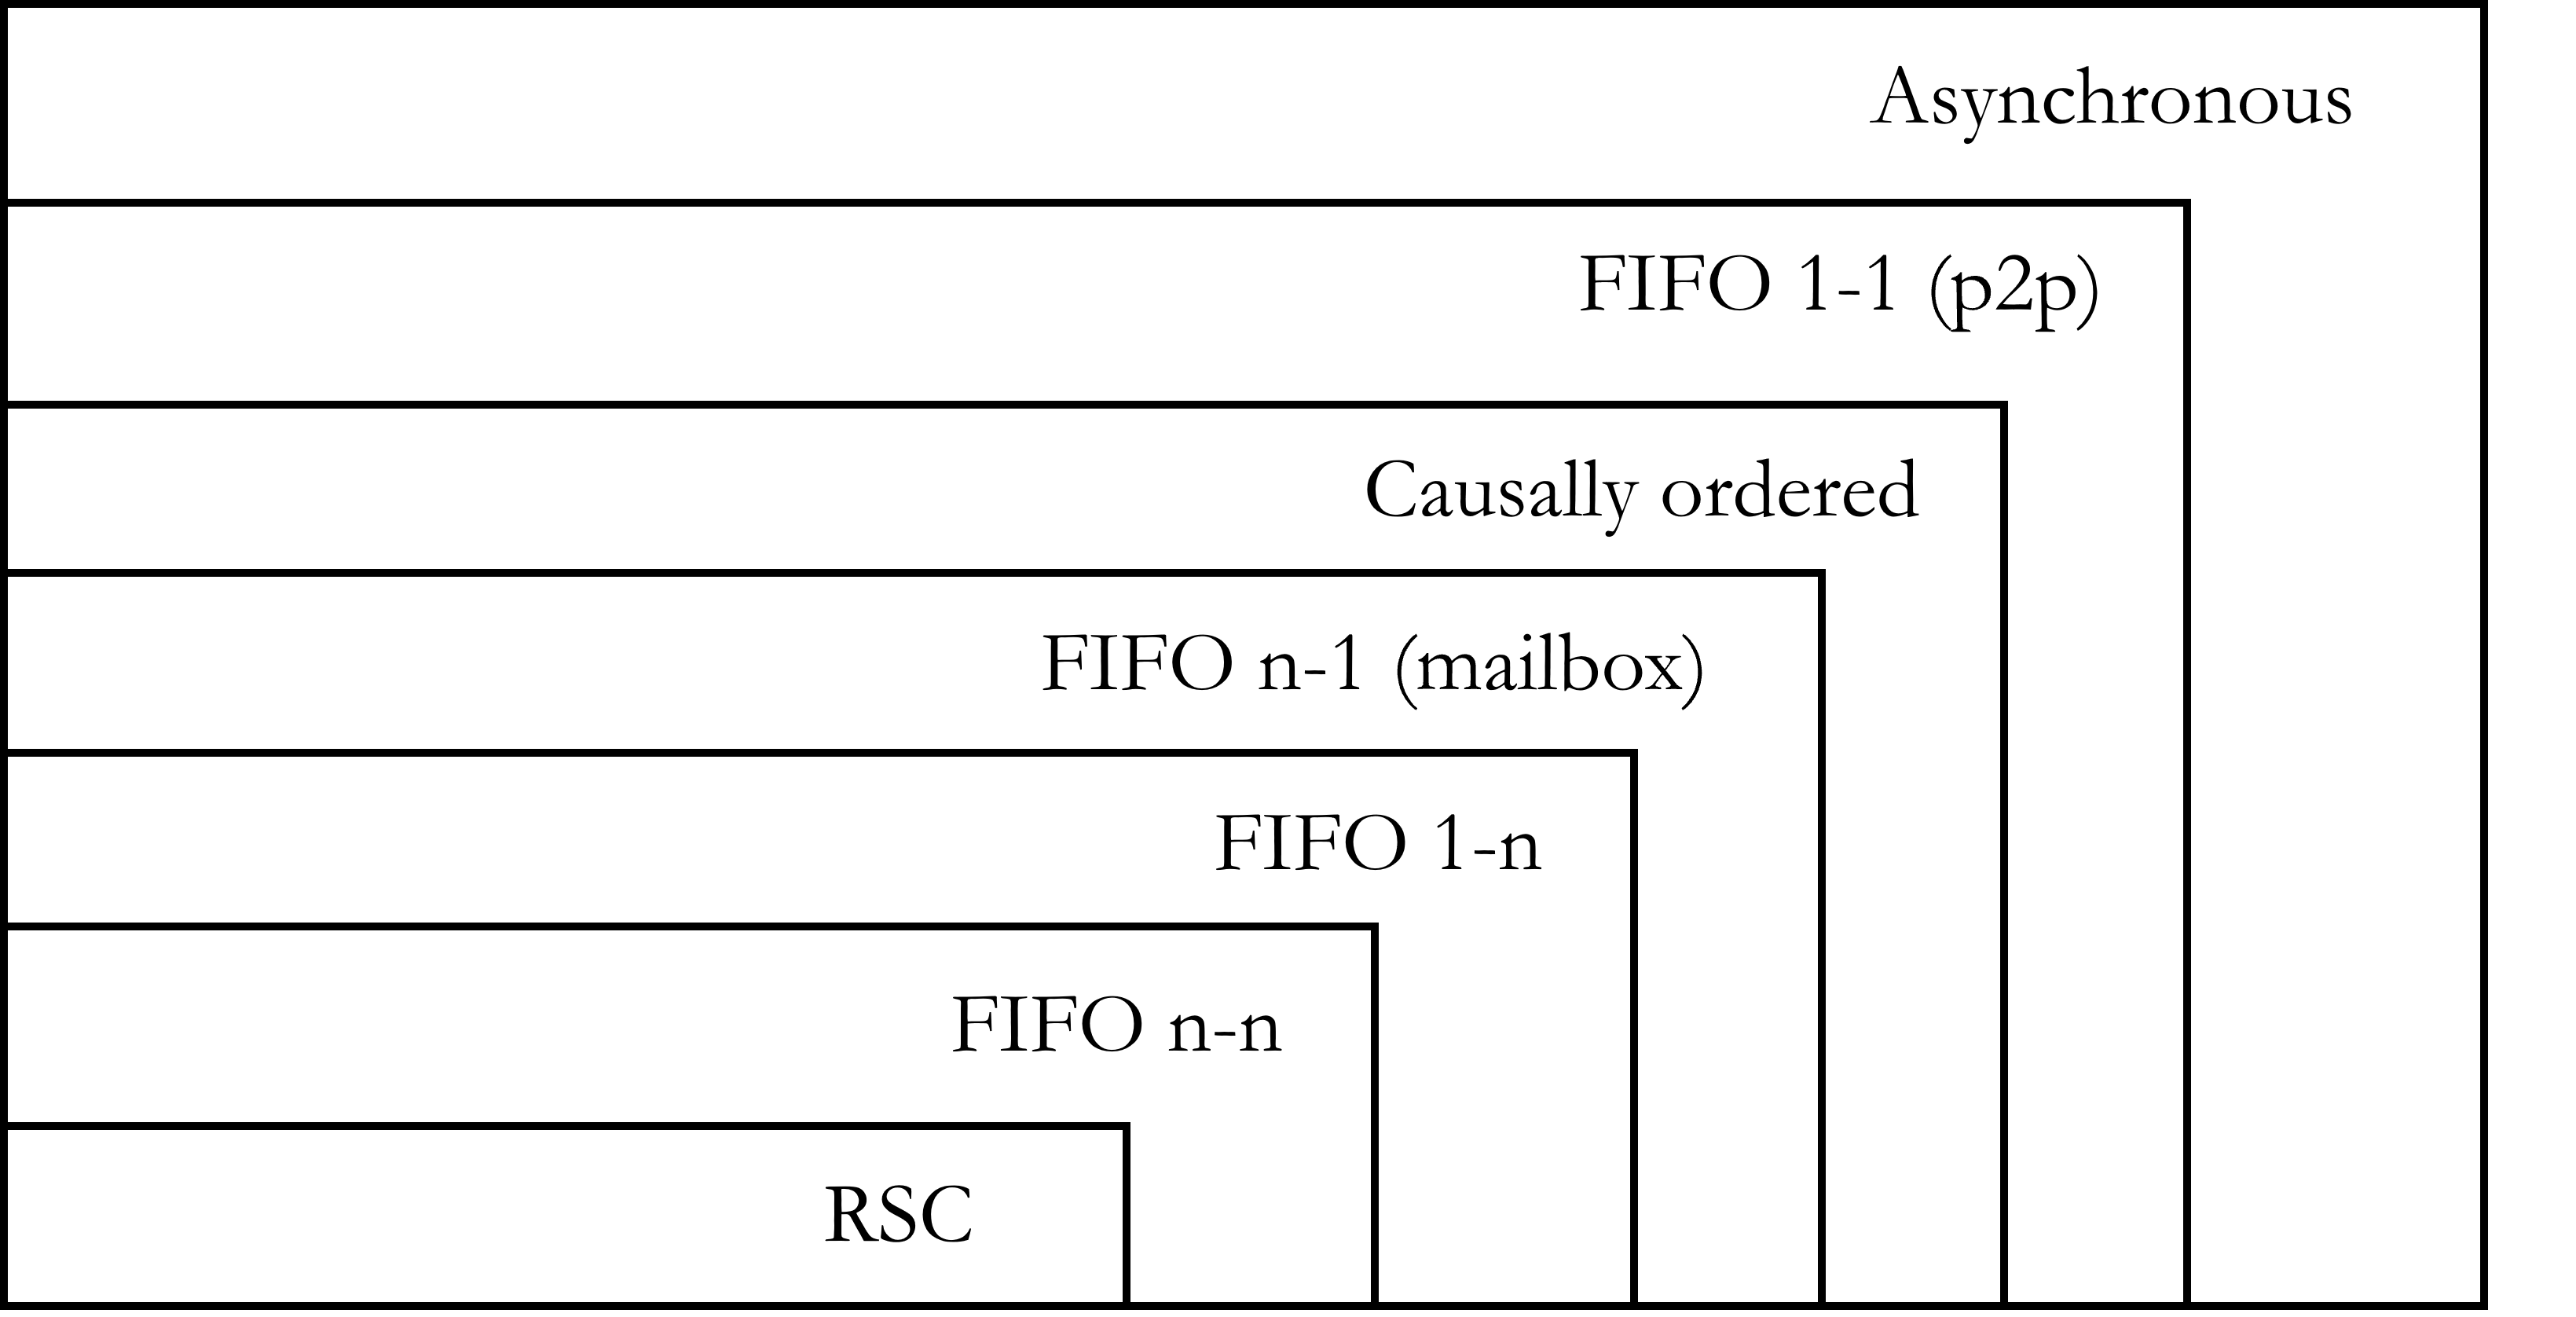
\includegraphics[width=8cm]{msc_hierarchy}
% 	\caption{The hierarchy of MSC classes.}
% 	\label{fig:msc_hierarchy_full}
% \end{figure}

\begin{figure}[h]
	\centering
	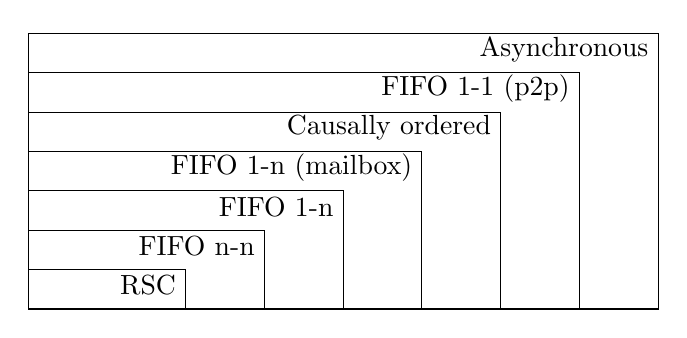
\begin{tikzpicture}
		\draw  (0,0) rectangle (2,.5);
		\draw (2,0.3) node[left]{RSC};
		\draw  (0,0) rectangle (3,1);
		\draw (3,0.8) node[left]{FIFO n-n};
		\draw  (0,0) rectangle (4,1.5);
		\draw (4,1.3) node[left]{FIFO 1-n};
		\draw  (0,0) rectangle (5,2);
		\draw (5,1.8) node[left]{FIFO 1-n (mailbox)};
		\draw  (0,0) rectangle (6,2.5);
		\draw (6,2.3) node[left]{Causally ordered};
		\draw  (0,0) rectangle (7,3);
		\draw (7,2.8) node[left]{FIFO 1-1 (p2p)};
		\draw  (0,0) rectangle (8,3.5);
		\draw (8,3.3) node[left]{Asynchronous};
	\end{tikzpicture}
	\caption{The hierarchy of MSC classes.}
	\label{fig:msc_hierarchy_full}
\end{figure}

\cinzia{add fig. of results}


\paragraph{Outline.} The paper is organized as follows. Next Section \ref{sec:com_models_overview} details the communication models we consider. Section \ref{sec:prelim} collects formal definitions that will be uses throughout the paper. Then Section \ref{sec:MSO} gives a formal definition of MSC realizing a given communication model and characterize the class of MSCs via MSO logic. Finally Sections \ref{sec:hierarchy} and \ref{sec:checking} show respectively how the different communication models are related and use this information to show some (un)decidability model checking results that follows from the notion of special treewidth.

